\section{Homogeneous quadratics in $n$ variables}\label{sec:part1}
In this section we consider the case when $V = \F_p^n$ and $S \subset V$ is a quadric defined by
\[
	S = \{(x_1,\ldots,x_n) \mid Q(x_1,\ldots,x_n) = 0\}
\]
where $Q$ is a homogeneous quadratic. The set $S$ is conical because $Q$ is homogeneous, and in view of Lemma \ref{lem:FT-conical-subset}, our task is to determine $|\ker \xi \cap S|$ given a $\xi \in V^*$. If we write elements of $V$ as column vectors, then elements $\xi \in V^*$ can be represented as row vectors, with
\[
	\ker \xi = \langle \xi \rangle^\bot = \{x \in V \mid \xi x =0\}.
\]
Here $\langle \xi \rangle$ means the span of $\xi$.

We begin with an illustrative example over the reals before considering the situation over $\F_p$. Let $Q = 3x_1^2 + 3x_2^2 - 2x_3^2$.
The intersection $\langle \xi \rangle^\bot \cap S$ has three possible shapes:
\begin{itemize}
	\item a pair of lines intersecting at the origin (which is depicted in Figure~\ref{fig:conic-with-plane} with $\xi = (0,-2,1)$),
	\item the origin alone (e.g. $\xi = (0,0,1)$), and
	\item a single line, which happens when $\langle \xi \rangle^\bot$ is tangent to the quadric (e.g. $\xi = (0,-\sqrt{3},\sqrt{2})$).
\end{itemize}
\begin{figure}[h]
	\centering
	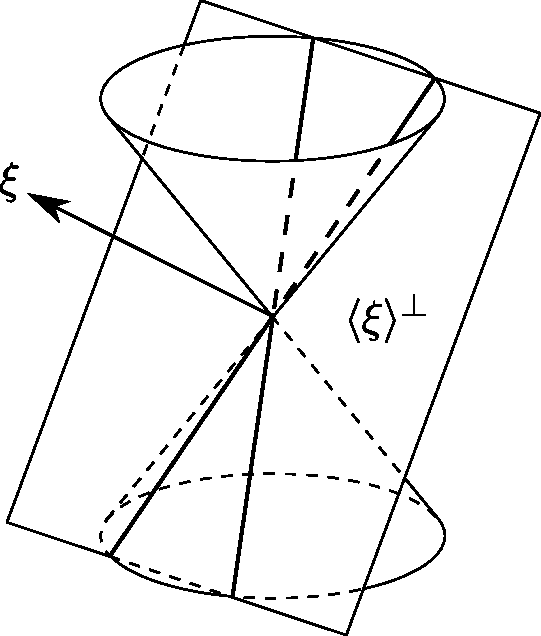
\includegraphics[width=0.6\linewidth]{conic-with-plane}
	\caption{Over the reals, when $\xi=(0,-2,1)$, the intersection of $S = \{3x_1^2 + 2x_2^2 - 2x_3^2 = 0\}$ with the hyperplane $\langle \xi \rangle^\bot$ is a pair of lines through the origin.}
	\label{fig:conic-with-plane}
\end{figure}
In fact, the set of $\xi$ such that $\langle \xi \rangle^\bot$ is tangent to the quadric is given by
\[
	\left\{ \xi = (\xi_1,\xi_2,\xi_3) \,\middle|\, \frac{1}{3} \xi_1^2 + \frac{1}{3} \xi_2^2 - \frac{1}{2} \xi_3^2 = 0 \right\} \subset V^*.
\]
This is a quadric in $V^*$, and it is dual to our original quadric in a sense that we will soon explain. Let us write $Q^*$ for the equation of this dual quadric. Observe that $Q^*(0,-2,1) > 0$ while $Q^*(0,0,1) < 0$. It turns out that the sign of $Q^*(\xi)$ is all one needs to classify the intersection $\langle \xi \rangle^\bot \cap S$. Equivalently, one needs only consider the existence of square-roots of $Q^*(\xi)$---a notion which, unlike ``sign,'' still makes sense over $\F_p$.

Now we consider the general situation in $n$ variables over a field $k$. We will require that $\operatorname{char} k \neq 2$, and that the product of two non-squares in $k$ is a square. The fields $\R$ and $\F_p$ for $p>2$ are examples. To a homogeneous quadratic
\[
	Q = \sum_{1 \leq i \leq j \leq n} c_{i,j} x_i x_j 
\]
we associate the $n\times n$ matrix $A$ whose entries are given by
\[
	a_{i,j} = \begin{cases}
		{c_{i,j}}/{2} & \text{if } i < j,\\
		c_{i,j} & \text{if } i = j, \text{ and}\\
		{c_{j,i}}/{2} & \text{if } i > j.
	\end{cases}
\]
Then, if $x = (x_1,\ldots,x_n)^\top$, we have
\[
	Q(x) = x^\top A x.
\]
The quadric $S = \{Q = 0\}$ is \emph{non-degenerate} if the matrix $A$ is invertible. We will assume that this is the case.

Suppose $g \in GL(V)$ is an invertible linear operator on $V$ such that $g(S) = S$; i.e. it induces a bijection of $S$ with itself. If $\xi \in V^*$, the identity $(g^\top \xi)^\top x = \xi^\top (gx)$ shows that $g$ also induces a bijection of $\langle g^\top \xi \rangle^\bot$ with $\langle \xi \rangle^\bot$. Therefore we obtain a bijection
\begin{equation}\label{eq:S-operator-hyperplane-bijection}
	g\colon S \cap \langle g^\top \xi \rangle^\bot \to S \cap \langle \xi \rangle^\bot.
\end{equation}
Our interest in these operators $g$ motivates the following definition.
\begin{defn}
	The \emph{orthogonal group of $A$}, denoted $O(A)$, is defined to be
	\[
		O(A) \coloneqq \{ g \in GL(V) \mid g^\top A g = A\}.
	\]
	Also define the \emph{conical orthogonal group of $A$} as
	\[
		kO(A) \coloneqq \{ cg \mid c\in k^\times, g\in O(A)\}.
	\]
\end{defn}
By construction, elements of $O(A)$ map $S$ bijectively to itself. Elements of $kO(A)$ do as well, because $S$ is conical. The action of $kO(A)$ on $V$ has another important feature which we now discuss. 
\begin{defn}
	A group $G$ acts \emph{transitively} on a set $X$ if for all $a,b\in X$, there exists $g\in G$ such that $g\cdot a = b$. Equivalently, the only orbit of the action is the entirety of $X$.
\end{defn}

\begin{prop}\label{prop:OA-transitive-action}
	The group $kO(A)$ acts transitively on each of the following sets:
	\begin{enumerate}
		\item $S_0(A) \coloneqq \{x \in V \mid x\neq 0, x^\top A x = 0\}$,
		\item $S_+(A) \coloneqq \{ x\in V \mid x^\top A x \text{ is a nonzero square in } k\}$, and
		\item $S_-(A) \coloneqq \{ x\in V \mid x^\top A x \text{ is not a square in } k\}$.
	\end{enumerate}
\end{prop}
\begin{proof}
	If $u,v\in V$ belong to the same set above, we can assume $u^\top A u = v^\top A v$ (as it can be achieved by scaling). For the set $S_-(A)$, this relies on our assumption that the quotient of two non-squares is a square in $k$.
	
	If $u$ and $v$ are linearly dependent then the result is immediate, so suppose otherwise. Take a basis $\{u,v,e_3,\ldots,e_n\}$ and apply Gram-Schmidt to it, obtaining an orthogonal basis $\{u, w_2, w_3, \ldots,w_n\}$. Now consider the basis
	\[
		\{u,v,w_3,\ldots,w_n\}
	\]
	which has the property that
	\[
		w_i^\top A u = w_i^\top A v = w_i^\top A w_j = 0 \text{ for all } i \neq j, \text{ and }\\
		u^\top A u = v^\top A v.
	\]
	It is straightforward to verify that the linear transformation which interchanges $u$ and $v$ while fixing $w_3,\ldots,w_n$ is an element of $O(A)$.
\end{proof}

%Note that left-multiplication by an element $g \in O(A)$ on $V$ induces right-multiplication by $g^{-1}$ on $V^*$.

Now suppose that $\xi^\top,\xi'^\top$ both belong to $S_0(A^{-1})$ (the following argument applies for the other two sets in Proposition \ref{prop:OA-transitive-action} as well). Then there exists $g \in O(A^{-1})$ such that $g \xi^\top = \xi'^\top$. If $\xi x = 0$, then
\[
	\xi' (g^\top)^{-1} x = \xi x = 0
\]
and thus $(g^\top)^{-1}$ maps $\langle \xi \rangle^\bot$ to $\langle \xi' \rangle^\bot$. Moreover, since $g \in O(A^{-1})$, inverting the identity $g^\top A^{-1} g = A^{-1}$ shows that $(g^\top)^{-1} \in O(A)$. Thus as in \eqref{eq:S-operator-hyperplane-bijection} we get a map
\[
	(g^\top)^{-1} \colon S \cap \langle \xi \rangle^\bot \to S \cap \langle \xi' \rangle^\bot
\]
which is a bijection.

Specializing back to $k=\F_p$ for $p>2$ a prime, this bijection implies that $|S \cap \langle \xi \rangle^\bot|$ depends only on whether $\xi$ belongs to $S_0(A^{-1})$, $S_+(A^{-1})$, or $S_-(A^{-1})$. By Lemma \ref{lem:FT-conical-subset}, the Fourier transform $\widehat{\IND_S}$ assumes only a few values, and we have proven the following theorem.

\begin{thm}\label{thm:FT-quadratic-constants-TBD}
	Let $p > 2$ be a prime and let $Q(x_1,\ldots,x_n)$ be a homogeneous non-degenerate quadratic. Write $S$ for the quadric $\{Q = 0\}$ in $V=\F_p^n$. Then,
	\begin{equation}
	\widehat{\IND_S}(\xi) = \begin{cases}
	\widehat{\IND_S}(0) & \text{if } \xi = 0,\\
	N_0 & \text{if } \xi \in S_0(A^{-1}),\\
	N_+ & \text{if } \xi \in S_+(A^{-1}), \text{ and}\\
	N_- & \text{if } \xi \in S_-(A^{-1}),
	\end{cases}
	\end{equation}
	for some constants $N_0$, $N_+$, and $N_-$.
\end{thm}
Let $Q^*$ be the quadratic given by
\[
	Q^*(\xi) = \xi A^{-1} \xi^\top.
\]
Then the above equivalently states that for nonzero $\xi$, the value of $\widehat{\IND_S}(\xi)$ depends only on the number of square roots of $Q^*(\xi)$.

Now we compute the constants in Theorem \ref{thm:FT-quadratic-constants-TBD}. Note that an invertible matrix $P$ defines a change of coordinates, where in the new coordinates the equation of the quadric is $x^\top P^\top A P x = 0$. The following proposition then implies that we need only consider homogeneous quadratics of a very specific form.
\begin{prop}\label{prop:diag-to-two-forms}
	Let $A$ be a symmetric invertible matrix over $\F_p$. If $\det A$ is a square, then there exists an invertible $n\times n$ matrix $P$ such that $x^\top P^\top A P x = 0$ has the form
	\begin{equation}
	x_1^2 + x_2^2 + \cdots + x_n^2 = 0. \tag{Q1}\label{eq:Q1}
	\end{equation}
	Otherwise, suppose $\det A$ is not a square. Then there exists an invertible $n\times n$ matrix $P$ such that $x^\top P^\top A P x = 0$ has the form
	\begin{equation}
	rx_1^2 + x_2^2 + \cdots + x_n^2 = 0 \tag{Q2}\label{eq:Q2}
	\end{equation}
	where $r \in \F_p$ is not a square.
\end{prop}
\begin{proof}
	It is a well-known fact (see for example \cite[Prop.~42:1]{omeara}) that there exists an invertible matrix $B$ such that $B^\top A B$ is diagonal:
	\[
	x^\top B^\top A B x = c_1 x_1^2 + c_2 x_2^2 + \cdots + c_n x_n^2
	\]
	where all the $c_i$ are nonzero because we assumed $A$ to be invertible. Each $c_i$ is either a square or not, so we can assume that $c_1,\ldots,c_m$ are non-squares and $c_{m+1},\ldots,c_n$ are squares, for some $m$. This is achieved by choosing an appropriate permutation matrix $M$ and considering $x^\top (BM)^\top A BMx$.
	
	Let $r$ be the first non-square in the list $1,2,\ldots,p-1$. Then $r/c_1,\ldots,r/c_m$ and $1/c_{m+1},\ldots,1/c_n$ are squares, where we use the fact that the product of two non-squares is a square in $\F_p$. Moreover, $r-1$ is a square and $r \neq 1$, so we also know that $r-1 = s^2$ for some nonzero $s\in \F_p$. Define the $2\times 2$ matrix
	\[
		J = \begin{bmatrix}
			s/r & -1/r\\
			1/r & s/r
		\end{bmatrix}
	\]
	which is easily checked to be invertible.
	
	Now there are two cases, depending on $\det A$. Observe that
	\[
		\det (B^\top A B) = (\det B)^2 \det A
	\]
	and thus is a square if and only if $\det A$ is. Hence $m$ is even precisely when $\det A$ is a square. If this is the case, take
	\[
		P = BM
		\begin{bmatrix}
		\sqrt{r/c_1} & &\\
		& \ddots &\\
		&& \sqrt{1/c_n}
		\end{bmatrix}
		\begin{bmatrix}
			J & & &\\
			& J & &\\
			&& \ddots &\\
			&&& 0
		\end{bmatrix}
	\]
	where the last matrix has $m/2$ blocks equal to $J$ on the diagonal, followed by zeros. The reader can check that this choice of $P$ gives \eqref{eq:Q1}. If instead $\det A$ is not a square, we deduce that $m$ is odd, and we take
	\[
		P = BM
		\begin{bmatrix}
		\sqrt{r/c_1} & &\\
		& \ddots &\\
		&& \sqrt{1/c_n}
		\end{bmatrix}
		\begin{bmatrix}
		1&  & & &\\
		& J &&&\\
		&& J & &\\
		&&& \ddots &\\
		&&&& 0
		\end{bmatrix}
	\]
	where the last matrix starts with a $1$ on the diagonal, followed by $(m-1)/2$ blocks equal to $J$, and ends with zeros. This choice of $P$ gives \eqref{eq:Q2}.
\end{proof}

Hence \eqref{eq:Q1} and \eqref{eq:Q2} are the only two forms we need to consider. In Appendix \ref{sec:recursion-for-quadratic-solns} we give recursions $f_n, g_n$ for computing the number of solutions to such equations. We conclude this section by giving an example of how to compute the constants in Theorem \ref{thm:FT-quadratic-constants-TBD} from $f_n$ and $g_n$.

\begin{example}
	Suppose that $-1$ is a square mod $p$, and that our quadric $S$ is cut out by the equation $x^\top A x = 0$ where $\det A$ is a square. By Proposition \ref{prop:diag-to-two-forms}, we may instead consider the equivalent equation \eqref{eq:Q1}.
	
	The value $\widehat{\IND_S}(0)$ is the total number of points on the quadric, which in this case is $f_n (0)$:
	\[
		\widehat{\IND_S}(0) = f_n(0).
	\]
	To compute $N_0$, observe that \eqref{eq:Q1} is equivalent to
	\begin{equation}\label{eq:Q1-1equiv}
		-x_1^2 + x_2^2 + \cdots + x_n^2 = 0
	\end{equation}
	because $-1$ is a square. Consider $\xi = (1,1,0,0,\ldots,0)$. Its kernel is the hyperplane $\{x_1 + x_2 = 0\}$. Substituting $x_1 = -x_2$ into \eqref{eq:Q1-1equiv} gives
	\[
	x_3^2 + \cdots + x_n^2 = 0.
	\]
	This has $p f_{n-2}(0)$ solutions in the variables $x_2,\ldots,x_n$. Thus
	\[
	N_0 = \frac{p^2 f_{n-2}(0) - f_n(0)}{p-1}.
	\]
	To compute $N_+$, consider $\xi = (1,0,0,\ldots,0)$ whose kernel is the hyperplane $\{x_1 = 0\}$. Substituting this into \eqref{eq:Q1} gives
	\[
	x_2^2 + x_3^2 \cdots + x_n^2 = 0
	\]
	which has $f_{n-1}(0)$ solutions in the variables $x_2,x_3,\ldots,x_n$, and thus
	\[
	N_+ = \frac{p f_{n-1}(0) - f_n(0)}{p-1}.
	\]
	Finally, to compute $N_-$, we note that \eqref{eq:Q1} is also equivalent to the quadric
	\begin{equation}\label{eq:Q1rrequiv}
		rx_1^2 + rx_2^2 + x_3^2 + \cdots + x_n^2 = 0
	\end{equation}
	and we can take $\xi = (1,0,0,\ldots,0)$ and consider the intersection of its kernel with this quadric. Setting $\{x_1 = 0\}$ in \eqref{eq:Q1rrequiv} gives the equation
	\[
		rx_2^2 + x_3^2 + \cdots + x_n^2 = 0
	\]
	which has $g_{n-1}(0)$ solutions, and hence
	\[
		N_- = \frac{pg_{n-1}(0) - f_n(0)}{p-1}.
	\]
	If $n$ is even, then $f_{n-1}(0) = g_{n-1}(0)$ (c.f. Appendix \ref{sec:recursion-for-quadratic-solns}) and thus $N_+ = N_-$.
\end{example}

We have seen that, for a non-degenerate homogeneous quadric $S = \{x^\top A x = 0\}$, the Fourier transform $\widehat{\IND_S}$ at $\xi\in V^*$ is closely related to the value of $\xi^\top A^{-1} \xi$. Specifically, nonzero elements of $V^*$ lying on the dual quadric $\{\xi^\top A^{-1} \xi = 0\}$ represent hyperplanes which are tangent to $S$. All tangent hyperplane cross-sections of $S$ look the same, although there may be two types of generic (non-tangent) hyperplane cross-sections. The cardinalities of these cross-sections are recorded by $\widehat{\IND_S}$.